\begin{corollary}
    Пусть выполняются условия регулярности (R0)-(R4), и $\displaystyle \forall n\in \mathbb{N} \ \forall X_{1} ,\ \dotsc ,\ X_{n}$ существует и единственно решение $\displaystyle \hat{\theta }_{n}( X_{1} ,\ \dotsc ,\ X_{n})$ уравнения правдоподобия, которое является статистикой. Тогда $\displaystyle \hat{\theta }_{n}$ -- состоятельная оценка $\displaystyle \theta $ и с вероятностью стремящейся к единице $\displaystyle \hat{\theta }$ является ОМП.
\end{corollary}
\begin{proof}
    Первая часть следует из доказательства предыдущей теоремы, т.к. $\displaystyle \hat{\theta }_{n}$ является измеримой функцией, которая не зависит от $\displaystyle \theta _{0}$. Также, из доказательства предыдущей теоремы событие
    
    
    \begin{gather*}
    S_{n} =\{x:\ f_{\theta _{0} -\varepsilon }( X_{1} ,\ \dotsc ,\ X_{n}) < f_{\theta _{0}}( X_{1} ,\ \dotsc ,\ X_{n}) ,\\
    f_{\theta _{0}}( X_{1} ,\ \dotsc ,\ X_{n})  >f_{\theta _{0} +\varepsilon }( X_{1} ,\ \dotsc ,\ X_{n})\} ,
    \end{gather*}
    где $\displaystyle \theta _{0}$ -- истинное значение параметра, выполняется с вероятностью, стремящейся к единице.
    
    
    
    
    
    
    \tikzset{every picture/.style={line width=0.75pt}} %set default line width to 0.75pt        
    
    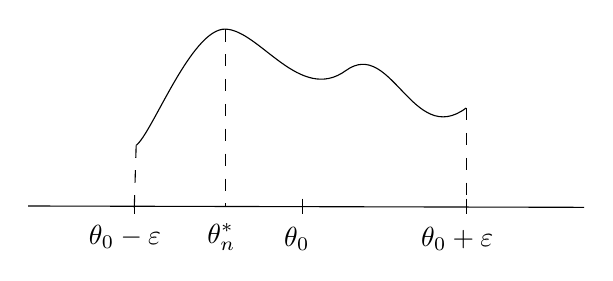
\begin{tikzpicture}[x=0.75pt,y=0.75pt,yscale=-1,xscale=1]
    %uncomment if require: \path (0,133); %set diagram left start at 0, and has height of 133
    
    %Straight Lines [id:da5523153205088052] 
    \draw    (198,93) -- (465.8,93.64) ;
    %Straight Lines [id:da26603836690721816] 
    \draw    (249,89.44) -- (249,97) ;
    %Straight Lines [id:da4784853099881268] 
    \draw    (330,89.44) -- (330,97) ;
    %Straight Lines [id:da0957361640887564] 
    \draw    (409,89.44) -- (409,97) ;
    %Curve Lines [id:da762463644985083] 
    \draw    (250,63.77) .. controls (257.71,57.99) and (276.65,7.35) .. (293,7.77) .. controls (309.35,8.2) and (329,43.77) .. (351,27.77) .. controls (373,11.77) and (383.23,65.1) .. (409,45.77) ;
    %Straight Lines [id:da37125569801727853] 
    \draw  [dash pattern={on 4.5pt off 4.5pt}]  (250,63.77) -- (249,97) ;
    %Straight Lines [id:da08819979926603105] 
    \draw  [dash pattern={on 4.5pt off 4.5pt}]  (409,45.77) -- (409,89.44) ;
    %Straight Lines [id:da5655449448849437] 
    \draw  [dash pattern={on 4.5pt off 4.5pt}]  (293,7.77) -- (293,92.77) ;
    
    % Text Node
    \draw (320,102) node [anchor=north west][inner sep=0.75pt]   [align=left] {$\displaystyle \theta _{0}$};
    % Text Node
    \draw (386,102) node [anchor=north west][inner sep=0.75pt]   [align=left] {$\displaystyle \theta _{0} +\varepsilon $};
    % Text Node
    \draw (226,101) node [anchor=north west][inner sep=0.75pt]   [align=left] {$\displaystyle \theta _{0} -\varepsilon $};
    % Text Node
    \draw (283,100) node [anchor=north west][inner sep=0.75pt]   [align=left] {$\displaystyle \theta _{n}^{*}$};
    
    
    \end{tikzpicture}
    
    
    
    На отрезке $\displaystyle [ \theta _{0} -\varepsilon ,\ \theta _{0} +\varepsilon ]$ достигается максимум во внутренней точке $\displaystyle \theta _{n}^{*}$, и в ней $\displaystyle \frac{\partial f}{\partial \theta } =0$. Так как корень $\displaystyle \hat{\theta }_{n}$ единственный, то $\displaystyle \hat{\theta }_{n} =\theta _{n}^{*}$.
    
    Докажем, что $\displaystyle \hat{\theta }_{n}$ -- глобальный максимум. Предположим, что существует точка $\displaystyle \tilde{\theta }_{n}$, в которой значение функции $\displaystyle f$ не меньше, чем в $\displaystyle \hat{\theta }_{n}$. Тогда, между $\displaystyle \tilde{\theta }_{n}$ и $\displaystyle \hat{\theta }_{n}$ будет точка локального минимума, в которой $\displaystyle \frac{\partial f}{\partial \theta } =0$. Но это противоречие с условием единственности корня уравнения правдоподобия.
    
    Таким образом, $\displaystyle \hat{\theta }_{n}$ -- ОМП с большой вероятностью, т.е. на $\displaystyle S_{n}$.
\end{proof}
\begin{theorem}
    В условиях (R0)-(R8) любая состоятельная последовательность оценок $\displaystyle \hat{\theta }_{n}( X_{1} ,\ \dotsc ,\ X_{n})$, являющихся решениями уравнения правдоподобия, удовлетворяют соотношению
    \begin{equation*}
        \forall \theta \in \Theta \hookrightarrow \sqrt{n}(\hat{\theta }_{n} -\theta )\xrightarrow{d_{\theta }}\mathcal{N}\left( 0,\, \dfrac{1}{i( \theta )}\right) ,
    \end{equation*}
    где $\displaystyle i( \theta )$ -- количество информации Фишера в одном наблюдении.
\end{theorem}
\begin{proof}
    $\displaystyle L( X,\ \theta ) =\ln f_\theta(X)$. Применим формулу Тейлора в окрестности точки $\displaystyle \theta _{0}$:
    \begin{equation*}
        0=L^{'}( X,\ \hat{\theta }_{n}) =L^{'}( X,\ \theta _{0}) +(\hat{\theta }_{n} -\theta _{0}) L^{''}( X,\ \theta_0) +\dfrac{(\hat{\theta }_{n} -\theta _{0})^{2}}{2} L^{'''}\left( X,\ \theta _{n}^{*}\right) ,
    \end{equation*}
    где $\displaystyle \theta _{n}^{*}$ лежит между $\displaystyle \theta _{0}$ и $\displaystyle \hat{\theta }_{n}$. Тогда 
    \begin{equation*}
        \sqrt{n}(\hat{\theta }_{n} -\theta _{0}) =\dfrac{\frac{L^{'}( X,\ \theta _{0})}{\sqrt{n}}}{-\frac{1}{n} L^{''}( X,\ \theta _{0}) -\frac{1}{2n}(\hat{\theta }_{n} -\theta _{0}) L^{'''}\left( X,\ \theta _{n}^{*}\right)} .
    \end{equation*}
    Покажем, что $\displaystyle \dfrac{1}{\sqrt{n}} L'( X,\ \theta _{0})\xrightarrow{d_{\theta }}\mathcal{N}( 0,\ i( \theta _{0}))$, где $\displaystyle i( \theta _{0})$ -- информация Фишера одного наблюдения. Рассмотрим
    \begin{equation*}
        \dfrac{1}{\sqrt{n}} L^{'}( X,\ \theta _{0}) =\dfrac{1}{\sqrt{n}}\sum _{k=1}^{n}\dfrac{f^{'}_{\theta _{0}}( X_{k})}{f_{\theta _{0}}( X_{k})} .
    \end{equation*}
    Под знаком суммы независимые, одинаково распределенные случайные величины. В доказательстве неравенства Рао-Крамера было доказано, что $\displaystyle E_{\theta _{0}}\dfrac{f^{'}_{\theta _{0}}( X_{k})}{f_{\theta _{0}}( X_{k})} =0$, и \ $\displaystyle D_{\theta _{0}}\dfrac{f^{'}_{\theta _{0}}( X_{k})}{f_{\theta _{0}}( X_{k})} =i( \theta _{0})$. Следовательно, по ЦПТ получаем требуемое.
    Также,
    \begin{equation*}
        -\dfrac{1}{n} L^{''}( X,\ \theta _{0}) =\dfrac{1}{n}\sum _{k=1}^{n}\dfrac{\left( f_{\theta _{0}}^{'}( X_{k})\right)^{2} -f_{\theta _{0}}( X_{k}) f_{\theta _{0}}^{''}( X_{k})}{f_{\theta _{0}}^{2}( X_{k})}\xrightarrow{P_{\theta _{0}}} I( \theta _{0}) -E_{\theta _{0}}\left(\dfrac{f_{\theta _{0}}^{''}( X_{1})}{f_{\theta _{0}}( X_{1})}\right) =i( \theta _{0}) ,
    \end{equation*}
    так как $\displaystyle E_{\theta _{0}}\left(\dfrac{f_{\theta _{0}}^{''}( X_{1})}{f_{\theta _{0}}( X_{1})}\right) =\int _{A}\dfrac{f_{\theta _{0}}^{''}( x)}{f_{\theta _{0}}( x)} f_{\theta _{0}}( x) dx=\int _{A} f_{\theta _{0}}^{''}( x) dx=\left(\int _{A} f_{\theta _{0}}( x)dx\right)^{''} =1^{''} =0$.
    
    Докажем, что величина $\displaystyle \dfrac{1}{n} L^{'''}\left( X,\ \theta _{n}^{*}\right)$ ограничена по вероятности. Так как оценка $\displaystyle \hat{\theta }_{n}$ состоятельна, то с вероятностью, стремящейся к единице $\displaystyle \theta _{n}^{*}$ лежит в малой окрестности $\displaystyle \theta _{0}$, а значит применимо условие (R8):
    \begin{equation*}
        \left| \dfrac{1}{n} L^{'''}\left( X,\ \theta _{n}^{*}\right)\right| \leq \dfrac{1}{n}\sum _{k=1}^{n} H( X_{k}) ,
    \end{equation*}
    где неравенство выполняется с вероятностью, стремящейся к единице. Также,
    \begin{equation*}
        \dfrac{1}{n}\sum _{k=1}^{n} H( X_{k})\xrightarrow{P_{\theta _{0}}} E_{\theta _{0}} H( X_{1}) .
    \end{equation*}
    Значит, $\displaystyle \dfrac{1}{n} L^{'''}\left( X,\ \theta _{n}^{*}\right)$ ограничена по вероятности. Из этого следует, что
    \begin{equation*}
        \frac{1}{n}(\hat{\theta }_{n} -\theta _{0}) L^{'''}\left( X,\ \theta _{n}^{*}\right)\xrightarrow{P_{\theta _{0}}} 0.
    \end{equation*}
    Следовательно,
    \begin{equation*}
        -\frac{1}{n} L''( X,\ \theta _{0}) -\frac{1}{2n}(\hat{\theta }_{n} -\theta _{0}) L'''\left( X,\ \theta _{n}^{*}\right)\xrightarrow{P_{\theta _{0}}} i( \theta _{0}) .
    \end{equation*}
    Тогда
    
    \begin{equation*}
        \dfrac{\frac{L'( X,\ \theta _{0})}{\sqrt{n}}}{-\frac{1}{n} L''( X,\ \theta _{0}) -\frac{1}{2n}(\hat{\theta }_{n} -\theta _{0}) L'''\left( X,\ \theta _{n}^{*}\right)}\xrightarrow{d_{\theta _{0}}}\mathcal{N}\left( 0,\ \dfrac{1}{i( \theta _{0})}\right) .
    \end{equation*}
\end{proof}
\begin{note}
    Формально перенеся $\displaystyle \sqrt{n}$ в правую часть, получим, что асимптотическая дисперсия будет равняться информации Фишера всей выборки. Таким образом, эту теорему можно воспринимать, как асимптотическую версию неравенства Рао-Крамера.
\end{note}
\begin{corollary}
    (асимптотическая нормальность ОМП) В условиях (R0)-(R8), если $\displaystyle \forall n\in \mathbb{N} \ \forall X_{1} ,\ \dotsc ,\ X_{n}$ существует единственное решение $\displaystyle \hat{\theta }_{n}$ уравнения правдоподобия, и если оно является статистикой, то $\displaystyle \hat{\theta }_{n}$ -- асимптотически нормальная оценка $\displaystyle \theta $ с асимптотической дисперсией $\displaystyle \dfrac{1}{i( \theta )}$ и с вероятностью, стремящейся к единице, является ОМП. 
\end{corollary}
\begin{theorem}
    (Бахадур, б/д) Пусть выполнены условия регулярности (R0)-(R8), и $\displaystyle \hat{\theta }_{n}( X_{1} ,\ \dotsc ,\ X_{n})$ асимптотически нормальная оценка $\displaystyle \theta $, т.е. $\displaystyle \sqrt{n}(\hat{\theta }_{n} -\theta )\xrightarrow{d_{\theta }}\mathcal{N}\left( 0,\ \sigma ^{2}( \theta )\right)$, причем $\displaystyle \sigma ( \theta )$ непрерывна. Тогда, $\displaystyle \forall \theta \in \Theta \hookrightarrow \sigma ^{2}( \theta ) \geqslant \dfrac{1}{i( \theta )}$.
\end{theorem}
\begin{note}
    Эта теорема также является некоторой асимптотической версией неравенства Крамера-Рао.
\end{note}
\begin{corollary}
    В условиях следствия про асимптотическую нормальность ОМП имеем, что ОМП не хуже любой другой оценки в асимптотическом подходе в классе оценок с непрерывной дисперсией.
\end{corollary}
\begin{definition}
    Если $\displaystyle \sqrt{n}(\hat{\theta }_{n}( X_{1} ,\ \dotsc ,\ X_{n}) -\theta )\xrightarrow{d_{\theta }}\mathcal{N}\left( 0,\ \dfrac{1}{i( \theta )}\right)$, то $\displaystyle \hat{\theta }_{n}$ называется асимптотически эффективной оценкой $\displaystyle \theta $.
\end{definition}
\begin{proposition}
    Пусть выполнены условия регулярности для неравенства Крамера-Рао, $\displaystyle \hat{\theta }( X)$ -- эффективная оценка $\displaystyle \theta $, и равенство из критерия эффективности (для $\displaystyle \hat{\theta }( X)$) выполнено для любого $\displaystyle X$ и любого $\displaystyle \theta $. Тогда $\displaystyle \hat{\theta }$ -- ОМП.
\end{proposition}
\begin{proof}
    По неравенству Крамера-Рао $\displaystyle \hat{\theta }( X) -\theta =\dfrac{1}{I_{X}( \theta )}\left(\dfrac{\partial }{\partial \theta }\ln f_{\theta }( X)\right)$. Тогда, если $\displaystyle \theta < \hat{\theta }( X)$, то $\displaystyle \dfrac{\partial }{\partial \theta }\ln f_{\theta }( X)  >0\Rightarrow f_{\theta }( X)$ возрастает. Если же $\displaystyle \theta  >\hat{\theta }( X)$, то $\displaystyle f$ убывает. Следовательно, максимум функции правдоподобия достигается в точке $\displaystyle \hat{\theta }( X)$.
\end{proof}
\section{Линейная регрессионная модель}

В линейной модели наблюдение -- случайный вектор $\displaystyle X\in \mathbb{R}^{n}$, который представляется в виде $\displaystyle X=l+\varepsilon $, где $\displaystyle l$ -- неслучайный неизвестный вектор, а $\displaystyle \varepsilon $ -- случайный вектор. Тогда, $\displaystyle l$ является оцениваемой величиной, а $\displaystyle \varepsilon $ трактуется как вектор ошибок. Будем считать, что $\displaystyle E\varepsilon =0,\ D\varepsilon =\sigma ^{2} I_{n},\ \sigma^2 > 0$, при этом $\displaystyle \sigma ^{2}$ неизвестен. Про $\displaystyle l$ известно, что $\displaystyle l\in L$, где $\displaystyle L$ -- линейное подпространство в $\displaystyle \mathbb{R}^{n}$. Задача состоит в оценивании $\displaystyle l$ и $\displaystyle \sigma ^{2}$.

Пусть $\displaystyle L$ задано с помощью базиса $\displaystyle ( Z_{1} ,\ \dotsc ,\ Z_{k})$ из вектор-столбцов. Следовательно, $\displaystyle \dim L=k$. Составим матрицу $\displaystyle Z=\begin{pmatrix}
Z_{1} & \dotsc  & Z_{k}
\end{pmatrix}$. Тогда, $\displaystyle l=Z\theta $, где $\displaystyle \theta $ -- вектор неизвестных координат в базисе $\displaystyle ( Z_{1} ,\ \dotsc ,\ Z_{k})$.

Таким образом, задача сведена к оцениванию $\displaystyle \left( \theta ,\ \sigma ^{2}\right) ,\ \theta \in \mathbb{R}^{k}$.
\subsection{Метод наименьших квадратов}
\begin{definition}
    Оценка по методу наименьших квадратов для линейной регрессионной модели для параметра $\displaystyle \theta $ -- это оценка
    \begin{equation*}
        \hat{\theta } =\arg\min_{\theta }\Vert X-Z\theta \Vert _{2}^{2} =\arg\min_{\theta }\langle X-Z\theta ,\ X-Z\theta \rangle .
    \end{equation*}
\end{definition}
\begin{note}
    $\displaystyle Z\hat{\theta }$ является проекцией вектора $\displaystyle X$ на подпространство $\displaystyle L$, т.е. $\displaystyle Z\hat{\theta } =proj_{L} X$.
\end{note}
\begin{lemma}
    $\displaystyle \hat{\theta } =\left( Z^{T} Z\right)^{-1} Z^{T} X$, где $\displaystyle \hat{\theta }$ -- оценка МНК параметра $\displaystyle \theta $.
\end{lemma}
\begin{proof}
    Так как функция $\displaystyle \Vert X-Z\theta \Vert _{2}^{2}$ выпукла, то в минимум достигается в ее точке стационарности. Путем дифференцирования выражения $\displaystyle ( X-Z\theta )^{T}( X-Z\theta ) =0$ и, выражая $\displaystyle \theta $, получаем требуемое.
\end{proof}
\begin{note}
    $\displaystyle Z^{T} Z$ является матрицей Грама, поэтому она обратима.
\end{note}